%-------------------------------------------------------------------------------
% Copyright (c) 2013-2016 University of Luxembourg.
% All rights reserved. This program and the accompanying materials
% are made available under the terms of the Eclipse Public License v1.0
% which accompanies this distribution, and is available at
% http://www.eclipse.org/legal/epl-v10.html
% 
% Contributors: 
%     Alfredo Capozucca - initial writing 
%      
%-------------------------------------------------------------------------------
%%%%%%%%%%%%%%%%%%%%%%%%%%%%%%%%%%%%%%%%%%%%%%%%%%
\PassOptionsToPackage{usenames,svgnames,table}{xcolor}
\documentclass[graybox,envcountchap,sectrefs]{./../lu.uni.lassy.excalibur.standard.report.libraries/styles/svmono}  
%%%%%%%%%%%%%%%%%%%%%%%%%%%%%%%%%%%%%%%%%%%%%%%%%%
%%% DO NOT CHANGE THE ORDER 
\usepackage{./../lu.uni.lassy.excalibur.standard.report.libraries/styles/style-messir-common}
\usepackage{./../lu.uni.lassy.excalibur.standard.report.libraries/styles/style-messir-report-post}
\usepackage{breakurl} 
%--------------------------------------------
 
% DOCUMENT BEGIN
%--------------------------------------------
\begin{document}

\newgeometry{textwidth=17cm,textheight=23.7cm}  
 
\input{./../lu.uni.lassy.excalibur.standard.report.libraries/defs/msr-def.tex}
\DeclareRobustCommand{\mysystemname}{myCrashVariant~}
\newglossaryentry{Concept Model}
{name={Concept Model},
description={the Model that describes the different types required to specify
the software system.}, 
plural={Concept Models},
symbol={\msrglsstyle{Concept Model}}
}

\newglossaryentry{Environment Model} 
{name={Environment Model},
description={the Model that describes the different actors supposed to interact
with the software system.}, 
plural={Environment Models},
symbol={\msrglsstyle{Environment Model}}
}



\newglossaryentry{MVC} 
{name={Model-View-Controller},
description={the pattern followed to design the Graphical User Interfaces
of the software system.}, 
plural={Model-View-Controllers}, 
symbol={\msrglsstyle{Model-View-Controller}}
}


\newglossaryentry{Design Model} 
{name={Design Model},
description={The Design Class Model is composed of the contents of all design classes, i.e.
their (value) attributes and methods, all the navigable associations between
design classes, and the inheritance structure. The Design Class Model has to be
modelled as a UML Class Diagram.}, 
plural={Design Models}, 
symbol={\msrglsstyle{Design Model}}
}


\newglossaryentry{Interaction Model} 
{name={Interaction Model},
description={The Interaction Model shows how objects are expected to interact at run-time to
support the \emph{system operations} specified in the \emph{Operation Model}
made during the Analysis Phase. There must exist an \emph{Interaction Model} for
each system operation specified in the \emph{Operation Model}. An Interaction Model has to be
modelled as a UML Sequence Diagram.}, 
plural={Interaction Models}, 
symbol={\msrglsstyle{Interaction Model}}
}

\newglossaryentry{Deployment View} 
{name={Deployment View},
description={The physical view depicts the system from a system engineer's
point-of-view. It is concerned with the topology of software components on the
physical layer, as well as the physical connections between these components.
For example, how many nodes are used and what is deployed on what node. A
Deployment View is modelled as a UML Deployment Diagram.}, 
plural={Deployment Views}, 
symbol={\msrglsstyle{Deployment View}}
}


\newglossaryentry{Implementation View} 
{name={Implementation View},
description={This view describes the software system components. It focuses on
software modules and subsystems. It describes the hierarchies or layers for
components. This view is modelled as a UML Component Diagram.},
plural={Implementation Views}, 
symbol={\msrglsstyle{Implementation View}}
}


\newglossaryentry{UI Processing View} 
{name={UI Processing View},
description={A Processing view is aimed at explaining the required
object interactions that allow a system operation to be called. A
UI Processing View is modelled as a UML Sequence Diagram.},
plural={UI Processing Views},
symbol={\msrglsstyle{UI Processing View}} }


\newglossaryentry{iCrash.FX} 
{name={iCrash Distributed Desktop development},
description={Implementation of the \msricrash case study made in \emph{Java} and
capable of ensuring a distributed execution.},
symbol={\msrglsstyle{iCrash.FX}} }





%  General Messir Glossary
\newglossaryentry{real number}
{name={Real number},
description={name of the set of real numbers.},
plural={reals},
symbol={\ensuremath{\mathbb{R}}}
}

\newglossaryentry{system operation}
{name={System Operation},
description={a functionality of the system that can be triggered by a message
sent by an actor belonging to the environment.}, plural={system operations},
symbol={\msrglsstyle{system operation}}
}


\newglossaryentry{societics}
{name={Societics},
description={Represents the fields of hardware/software
systems used for the society extension.}, 
symbol={\msrglsstyle{societics}}
}

\newglossaryentry{direct actor}
{name={Direct Actor},
description={an actor that interacts directly with the system. It thus belongs
to the environment.},
plural={direct actors},
symbol={\msrglsstyle{direct actor}}
}

\newglossaryentry{indirect actor}
{name={Indirect Actor},
description={an actor that interacts indirectly with the system through a direct
actor.  It thus belongs the domain but not to the environment.}, 
plural={indirect actors},
symbol={\msrglsstyle{indirect actor}}
}

\newglossaryentry{abstract actor}
{name={Abstract Actor},
description={an actor that does not exist in real life.},
plural={abstract actors},
symbol={\msrglsstyle{abstract actor}}
}

\newglossaryentry{socext}
{name={Society extension},
description={The society obtained by grouping people using natural means
extended with artificial means.},
symbol={\msrglsstyle{societics}}
}

\newglossaryentry{usecase}
{name={Use case},
description={A use case describes a sequence of actions that provide something
of measurable value to an actor. and is drawn as a horizontal ellipse.},
plural={Use cases}, 
symbol={\msrglsstyle{Use case}} 
}

\newglossaryentry{actor}
{name={Actor},
description={An actor is a person, organization, or external system that plays a
role in one or more interactions with the system.},
plural={actors},
symbol={\msrglsstyle{actor}}
}

\newglossaryentry{socialware}
{name={Societics},
description={Represents the fields of hardware/software
systems used for the society extension.},
symbol={\msrglsstyle{Societics}}
}

\newglossaryentry{myTerm}
{name={My Term},
description={Represents the simple glossary term},
symbol={\msrglsstyle{My Term}}
}


% \newglossaryentry{}
% {name={\msrglsstyle{}},
% description={},
% symbol={\msrglsstyle{actor}} }


%TITLE
%******************************************
\title{
\begin{tabular}{|>{\centering\arraybackslash\hspace{0pt}}p{16cm}|}
\hline
	\textbf{\emph{\mysystemname}}\\
	\textbf{Design Document}\\
	\textbf{ - v 0.0.5 - }\\
\hline 
\end{tabular}
\vspace{2cm}}
 
%******************************************
\author{
\begin{tabular}{l}
		Rafael Valiev\\
		Kasatkin Timur\\
		Gregory Yermolaev\\
		\\Innopolis University\\
\end{tabular}}

\date{\today~-~\currenttime}
%****************************************************


\maketitle
\newpage

%TOC
\setcounter{tocdepth}{2}
\addtocounter{secnumdepth}{2}
\tableofcontents
\newpage

%TOF
\listoffigures
\newpage

%TOL
\lstlistoflistings
\newpage

%DOCUMENT STRUCTURE

% Introduction
% Last Modification:
% @author AUTHOR_NAME
% @date TODAY_DATE

\chapter{Introduction}
\label{chap:introduction}

\section{Overview}

\section{Purpose and recipients of the document}

 
\section{Application Domain}

 
\section{Definitions, acronyms and abbreviations}


\section{Document structure} 

\newpage

% Analysis Models 
\chapter{Analysis Models}
\label{chap:AM}

This chapter provides a general overview of the main concepts gathered during
the analysis phase, in particular those concerning the software system types
(i.e. classes, datatypes, and enumerations), as well as the actors that interact
with the software system through their interfaces. Figures included in the
Messir Requirement Document that correspond to the  the \glspl{Concept Model} and the \glspl{Environment
Model} could be also included in this chapter, as a means of synthesizing what
are the requirements to which the design is supposed to sketch a solution.




\section{Concept Model}

%\usepackage{graphics} is needed for \includegraphics
\begin{figure}[H]
\begin{center}
  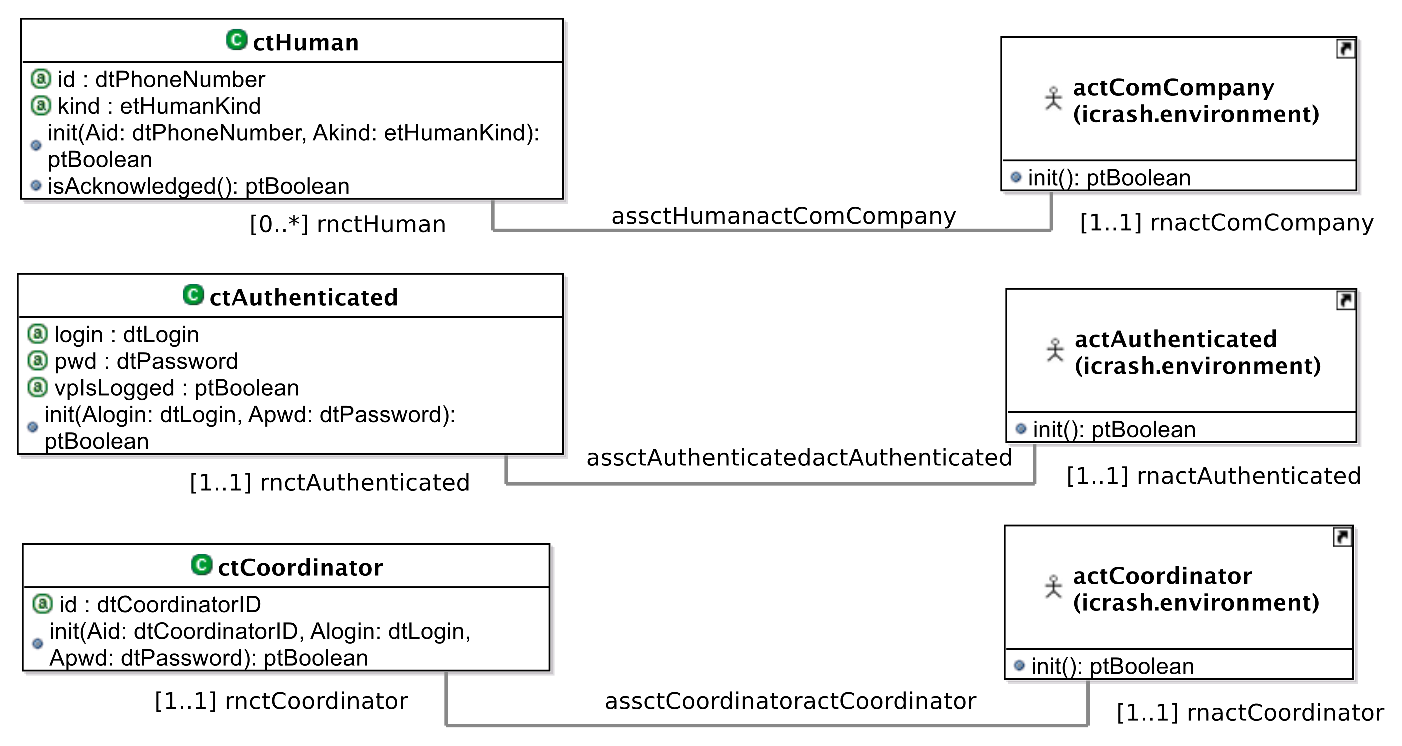
\includegraphics[width=400px]{images/analysis/concept-model/global/PrimaryTypes-Classes/01/cm-pt-ct-gv-01.eps}
  \caption{Concept Model - Primary types class types global view}
  \label{figureLabel}
\end{center}
\end{figure}

\subsection{Primary types - Class types descriptions}

\subsubsection{ctAuthenticated}
Used to model system’s representation about actors that need to authenticate to
access some specific functionalities.

\subsubsection{ctAdministrator}
Used to caracterize internally the entity that is responsible of administrating
the \mysystemname system.

\subsubsection{ctCoordinator}
Used to model system’s representation about the actors that have
the responsibility to handle alerts and crisis.

\subsubsection{ctCrisis} 
Used to model crisis that are infered from the reception of at least
one alert message. Crisis aer entities that are handled by the \mysystemname system.

\subsubsection{ctHuman} 
Used to model system’s representation about the indirect actors that has
alerted of potential crisis.

\subsubsection{ctAlert}
Used to model crisis alerts sent by any human having communication capability
using communication companies belonging to the system’s environment.

\subsubsection{ctState} 
Used to model the system. There is only one instance at any state of the
abstract machine after creation.

\subsection{Primary types - Datatypes types descriptions}

\subsubsection{Datatypes}

\paragraph*{\textbf{dtAlertID}}
A string used to identify alerts.

\paragraph*{\textbf{dtComment}}
A datatype made of a string value used to receive,store and send
textual information about crisis and alerts.

\paragraph*{\textbf{dtCoordinatorID}}
A string used to identify coordinators.

\paragraph*{\textbf{dtCrisisID}}
A string used to identify crisis.

\paragraph*{\textbf{dtGPSLocation}}
Used to define coordinates of geograpical positions on earth. It
is defined a couple made of a latitude and a longitude.

\paragraph*{\textbf{dtLatitude}}
Used to define a latitude value of a geograpical positions on earth.

\paragraph*{\textbf{dtLogin}}
A login string used to authentify an \mysystemname user

\paragraph*{\textbf{dtLongitude}}
Used to define a longitude value of a geograpical positions on
earth.

\paragraph*{\textbf{dtPassword}}
A password string used to authentify an \mysystemname user

\paragraph*{\textbf{dtPhoneNumber}}
A string used to store the phone number from the human declaring
the crisis or the alert.

\subsubsection{Enumerations}

\paragraph*{\textbf{etAlertStatus}} 
This type is used to indicate the different validation status of
an alert.

\paragraph*{\textbf{etCrisisStatus}} 
This type is used to indicate the different handling status of a
crisis.

\paragraph*{\textbf{etCrisisType}} 
This type is used to indicate the different types of a crisis.

\paragraph*{\textbf{etHumanKind}} 
This type is used to indicate the kind of human that informs about a
car crash crisis.

\subsection{Secondary types - Datatypes types descriptions}

\subsubsection{Datatypes}

\paragraph*{\textbf{dtSMS}}
A datatype made of a string value used to send textual information to human
mobile devices.

% \begin{figure}
% \begin{center}
% \includegraphics[width=\textwidth]{./images/myfigure.eps}
% \end{center}
% \caption{Caption for my figure}
% \label{fig:myfigure}
% \end{figure} 


   

\section{Environment Model}

%\usepackage{graphics} is needed for \includegraphics
\begin{figure}[H]
\begin{center}
  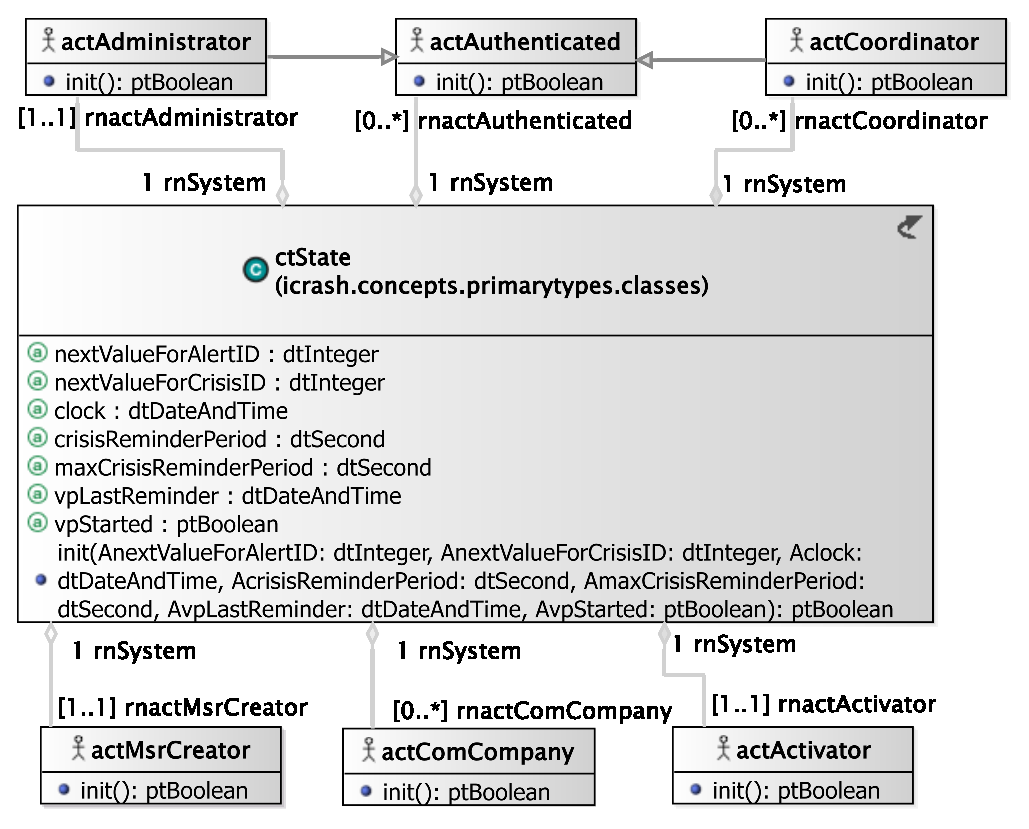
\includegraphics[width=400px]{images/analysis/environment-model/global/01/em-gv-01.eps}
  \caption{Environment Model - Global View}
  \label{env-global}
\end{center}
\end{figure}

\subsection{actMsrCreator Actor}
Represents the creator stakeholder in charge of state and environment
initialization.

\subsection{actActivator Actor}
Represents a logical actor for time automatic message sending based on system’s
or environment status.

\subsection{actAuthenticated Actor}
Abstract actor providing reusable input and output interfaces for actors that
need to authenticate themselves.

\subsection{actAdministrator Actor}
Represents an actor responsible of administration tasks for the \mysystemname
system. 

\subsection{actCoordinator Actor}
Represents actor responsible of handling one or several crisis for the
\mysystemname system.

\subsection{actComCompany Actor}
Represents the communication company stakeholder ensuring the input/ouput of
textual messages with humans having communication devices.

\newpage

% Technologies used to achieve the implementation
\chapter{Technological frameworks}
\label{chap:techFrm}


Provide a description of the technological frameworks used during the
development phase of your product. Such technological frameworks
should be properly introduced and described from the point of view of their
use during the development of your product.



\section{Tool 1}
\label{sec:Tool1}
It was required to \ldots


\section{Tool 2}
\label{sec:GUIDev}
It was required to \ldots




\newpage

% System architecture
\chapter{System Architecture}
\label{chap:arch}

This chapter presents information concerning the architecture of the software
system both from the static and dynamic viewpoints. The static viewpoint focuses
on the physical architecture (hardware) required to deploy and run the
software system along with the manner in which the components that make such
software system are grouped. On the other hand, the dynamic viewpoint focuses on
the behaviour of the software system at runtime. 

The static information is presented through the \gls{Deployment View} and the
\gls{Implementation View}. The dynamic aspects of the system are presented by
means of the \gls{UI Processing View}.


\section{Deployment view}
The aim of the \gls{Deployment View} is to describe the different processing nodes that compose
the deployment infrastructure and how they are interconnected. A processing node
corresponds to a piece of hardware aimed at executing either the whole software
system or a sub-part of it.




\section{Implementation view}
The \gls{Implementation View} describes each software system component and how
they are organised and combined to make the targeted software system.




\subsection{Component xx.yy.zz.c1}
TODO

\subsection{Component xx.yy.zz.c2}
TODO

\subsection{Component xx.yy.zz.c3}
TODO





\section{UI Processing view}
A \gls{UI Processing View} is aimed at explaining the required message exchanges
to achieve the launching of a system operation (specified in the \msrmessir
Analysis Document). These required message exchanges (which are not specified in
the \msrmessir Analysis Document) make part of the user interface (UI). Thus, the
main interest of a UI Processing View is to describe the design choices made
at the UI level, such that a system operation is launched. The description
of a UI Processing View is given by means of a UML Sequence Diagram. 


A complete Design Document should contain a UI Processing View for each
non-proactive system operation specified in the \msrmessir Analysis Document, as
such kind of system operations are launched by actors through UIs that allows
them to make so. 



\subsection{UI Processing view for system operation oeSystemOperation1}
TODO

 
\subsection{UI Processing view for system operation oeSystemOperation2}
TODO


\subsection{UI Processing view for system operation oeSystemOperation3}
TODO





\section{Non-functional runtime concerns}
The description of the runtime processes should be complemented with free
textual information regarding concurrency, distribution, performance and scalability aspects.


\subsection{Performance}
TODO



\subsection{Concurrency and Parallelism}
TODO




\subsection{Scalability}
TODO







\newpage

% Detailed Design
\chapter{Detailed design}
\label{chap:detDesign}


Provide an introduction to the proposed design. This introduction should help
the reader to understand the design choices made.


\section{Interaction Model}
An Interaction Model describes how each \gls{system operation} (that appears in the
Operation Model of the \msrmessir Requirements Analysis Model) is designed to meet
its specification. The design description of each system operation must be
focused on the messages exchanged between the different first-class objects
(i.e. instances of classes either included in Concept Model or introduced as
result of a design choice). An Interaction Model is modeled as a UML Sequence
Diagram.


\subsection{oeSystemOperation1}
TODO


\subsection{oeSystemOperation2}
TODO


\subsection{oeSystemOperation3}
TODO



\section{Design Class Model}
The Design Class Model is composed of the contents of all design classes (i.e.
every class appearing in at least one Interaction Model), all the navigable associations between design
classes, and the inheritance structure. The description of each class must
contain its attributes and operations. The Design Class Model is modeled as a
UML Class Diagram. 

It is advised to split the Design Class Model into multiple views as such model
may become pretty large. 
	

\subsection{Design Class Model view1}
TODO


\subsection{Design Class Model view2}
TODO



\subsection{Design Class Model view3}
TODO
\newpage

% Known limitations
\chapter{Known limitations}
\label{chap:know_limitations}


All known and non solved issues (like bugs, missing functionalities, abnormal
behavior, etc.) should be precisely stated and described.


\section{Issue 1}
TODO

\section{Issue 2}
TODO

\newpage


% Conclusion
\chapter{Conclusion}
\label{chap:final_conclusion}


TODO

\newpage

%APPENDICES
\appendix
% Here you add the appendices required for the design document

%\input{doc/appendix/appendix-1.tex} 

%\input{doc/appendix/appendix-2.tex} 

\newpage

%GLOSSARY
%Uncomment the line below if you want to print all glossaries no matter if they
% appear in the document
%\glsaddall
\printglossaries
\newpage

%BIBLIOGRAPHY
\cleardoublepage
\bibliographystyle{./../lu.uni.lassy.excalibur.standard.report.libraries/styles/lncs} 
\bibliography{./../lu.uni.lassy.excalibur.standard.report.libraries/defs/references/messir,doc/bibliography/design}
\label{sec:references}
 
\end{document}
